\section{Zeiten}

\subsection{Physikalische Zeit}

\subsubsection{Physikalische Zeit auf verschiedenen Rechnern}
Die physikalische Zeit stellt die uns im Alltag bekannte Uhrzeit dar. Die physikalische Zeit ist in vielen kryptographischen Verfahren von Bedeutung, da z.B. bestimmte Zertifikate (z.B. TSL) oder Authentifizierungen nur in einem bestimmten Zeitraum gültig sind. Deshalb ist ein genaues und sicheres Verfahren zur Bestimmung der physikalischen Zeit erwünscht.\\
Die physikalische Zeit, die wir auf einem Rechner haben wollen, ist die \textbf{Universal Time Coordinated (UTC)}, die auf internationaler Atomzeit basiert. Sie wird Weltweit über Kurzwelle oder Satellit ausgestrahlt. Aus der UTC kann man selbstverständlich die lokale Zeit errechnen.\\
Um sicherzustellen, dass jeder Rechner (oder andere Devices wie Smartphones oder IoT-Geräte) Zugriff zur UTC hat ist es naheliegend jeweils einen Atomzeitempfänger einzubauen. Da diese Empfänger aber zu teuer sind möchte man stattdessen nur wenige (spezielle) Rechner damit ausstatten und von dort aus die Zeit an alle anderen Rechner verteilen. Das Problem, dass sich ergibt, ist, dass Uhren in Rechnern nicht absolut genau laufen und deshalb periodisch synchronisiert werden müssen. Es stellt sich nun die Frage, wie ein Rechner damit umgehen soll, wenn er bei der Synchronisation feststellt, dass seine lokale Uhrzeit abgedriftet ist, also nichtmehr stimmt:
\begin{itemize}
    \item \textbf{lokale Uhr hängt hinterher:} In diesem Fall kann die lokale Zeit sofort angepasst werden und alle Events, die in dem übersprungenen Intervall gescheduled waren, werden sofort ausgeführt.
    \item \textbf{lokale Uhr ist zu weit:} In diesem Fall können wir die Uhr nicht zurückstellen, da sonst möglicherweise Events, die in dem dazwischenliegenden Zeitintervall gescheduled, waren doppelt ausgeführt werden würden. Demnach muss die lokale Uhr verlangsamt werden, also einige Ticks ausgesetzt werden, um die Korrektur durchzuführen.
\end{itemize}

Eine weitere Frage, die sich stellt, ist, wie oft diese Synchronisation durchgeführt werden sollte. Üblicherweise gibt der Hersteller des Geräts einen Wert $\rho$ an, der die maximale Abweichung nach einer bestimmten Zeiteinheit angibt. Daraus folgt, dass 2 verschiedene Uhren dieses Herstellers nach $\Delta t$ Zeiteinheiten eine maximale Abweichung $\delta = 2 \rho \Delta t$ Zeiteinheiten haben (, wenn die Uhr des einen Rechners maximal langsam und die des anderen maximal schnell lief). Durch Umstellen der Gleichung ergibt sich
\[ \Delta  t = \frac{\delta}{2 \rho}\]

Wir können uns nun eine maximale Abweichung $\delta$ überlegen, die wir erlauben wollen. Durch das Einsetzten in die Gleichung erhalten wir die Zykluslänge der Synchronisationen, die benötigt wird, um diese maximale Abweichung nicht zu überschreiten.

\subsubsection{Uhrabgleich - Christian\textquotesingle s Algorithm}

Der Christian\textquotesingle s Algorithm ist eine sehr simple Möglichkeit mehrere Rechner mit einem zentralen Zeitserver (der z.B. ein Atomzeitempfänger ist) abzugleichen. Das Verfahren ist wie folgt:
\begin{itemize}
    \item Jeder Client fragt zyklisch den zentralen Server nach seiner Uhrzeit
    \item Beim eintreffen der Nachricht berechnet der Client die Round Trip Time (RTT).
    \item Der Client addiert zur empfangenen Zeit die Hälfte der  RTT, um die Zeit, die für den Transfer benötigt wurde, auszugleichen und passt seine eigene Uhr an (verlangsamen oder Zeit übernehmen)
\end{itemize}

\subsubsection{Uhrabgleich - Berkeley Algorithm}

Der Berkeley Algorithmus ist ein einfaches Verfahren, um die Uhren von mehreren Rechnern zu synchronisieren. Dabei gibt es keinen Atomzeitempfänger und keinen Anspruch auf das Benutzen der wahren UTC. Stattdessen wird nur sichergestellt, das alle Rechner untereinander die gleiche Zeit haben (welche auch immer das dann ist). Das Verfahren ist wie folgt:
\begin{itemize}
    \item Ein zentraler Server fragt alle anderen Rechner zyklisch nach ihrer lokalen Zeit
    \item Der Server ermittelt den Mittelwert der lokalen Zeiten und sendet ihn an alle Rechner
    \item Die Rechner passen ihre lokale Zeit an den Mittelwert an
\end{itemize}

\subsubsection{Problem: beim Berkeley und Christian\textquotesingle s Algorithmus - Offset mit RTT bestimmen}
\label{sec:offset-with-rtt}

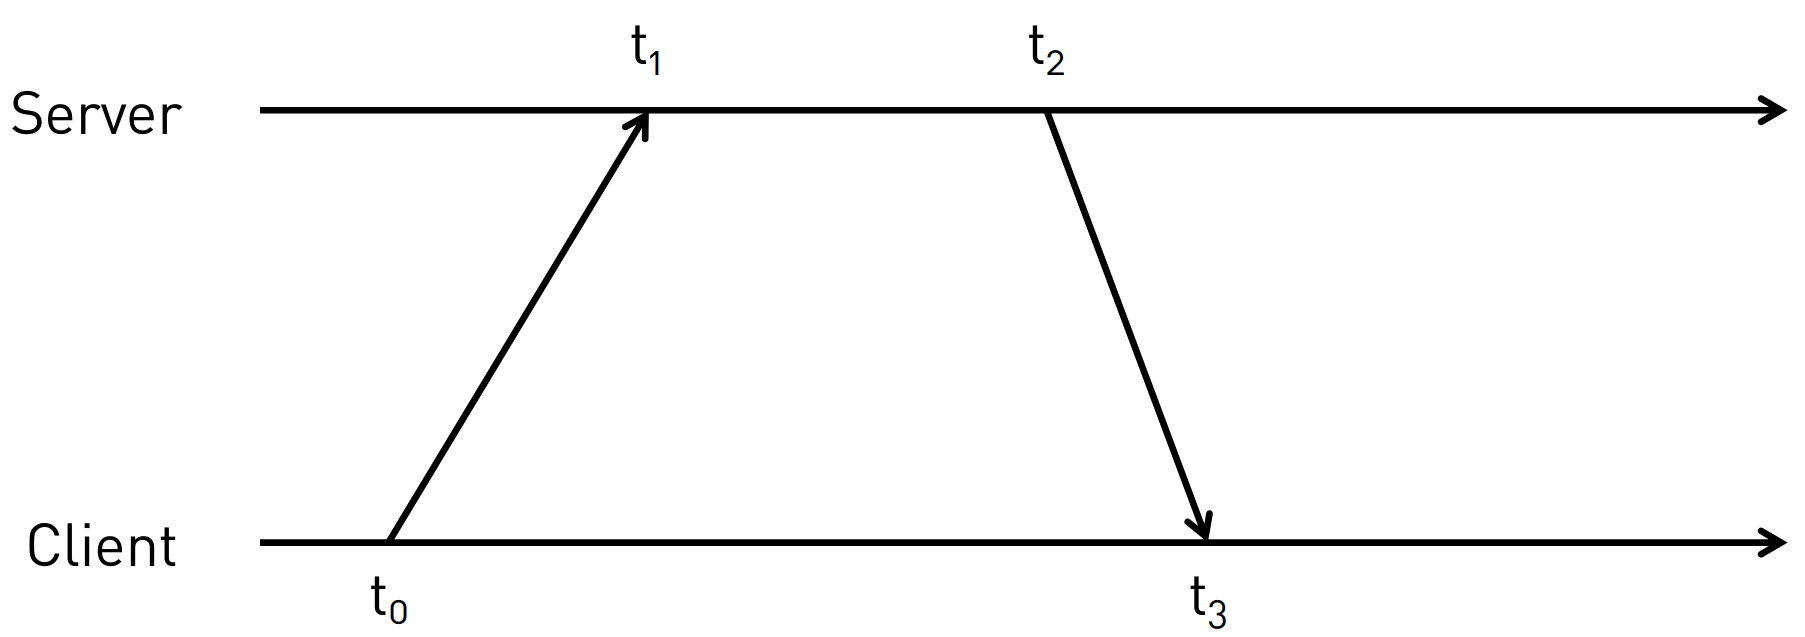
\includegraphics[height=130px]{RTT.png}

Wenn ein Rechner eine Zeit von einem Server gesendet bekommt, muss er beachten, dass diese schon wieder durch die Verzögerung des Netzwerks veraltet ist. Im Bild ist $t_{0}$ der Zeitpunkt an dem die Anfrage an den Zeitserver gesendet wird. Zum Zeitpunkt $t_{1}$ empfängt der Server die Anfrage und beantwortet sie zum Zeitpunkt $t_{2}$ mit der Zeit in diesem Moment. Der Client erhält diese Nachricht zu einem späteren Zeitpunkt $t_{3}$. Um die genaue Zeit auf dem Client zu bestimmen, müssten wir offensichtlich zur vom Server gesendeten Zeit die Übertragungszeit dieser Nachricht $\Delta t = t_{3} - t_{2}$ addieren. Das ist aber \textbf{nicht möglich}, da diese absoluten Zeiten von verschiedenen Uhren gemessen wurden und somit nicht vergleichbar sind. Stattdessen können wir nur jeweils die absoluten Zeiten $t_{0}$ und $t_{3}$, sowie $t_{1}$ und $t_{2}$ vergleichen. Somit können wir \textbf{nur näherungsweise} den Offset bestimmen:
\[
    O \approx \frac{t_{0} - t_{3} - (t_{2} - t_{1})}{2}
\]

\subsubsection{NTP - Network Time Protocol}

\vspace{5px}

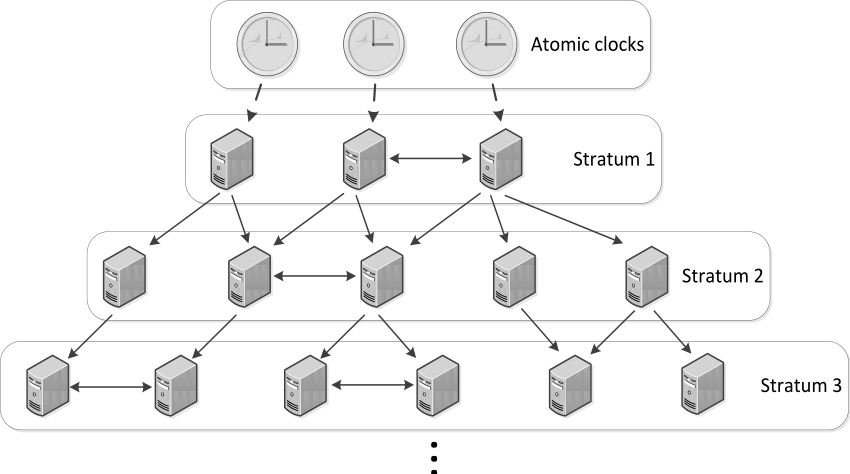
\includegraphics[height=170px]{NTP-typology.png}

Das Network Time Protocol (NTP) ist das Standardprotokoll zur Uhrensynchronisation im Internet. Dazu gibt es eine Reihe von Servern auf denen ein NTP-Daemon läuft. Die Topologie ist mehrschichtig in mehreren sogenannten Stratums aufgebaut, um skalierbar zu sein. Jeder Zeitserver aus Stratum $n$ ist ein Client (empfängt Zeit von Stratum $n-1$), ein Server (übermittelt Zeit zu Stratum $n+1$) und ein Peer (synchronisiert Zeit innerhalb Stratum $n$). Ein NTP-Daemon kann dabei auch mehrere Quellen abfragen und die \quotes{beste} Quelle wählen. Die Qualitätskriterien für Qualität eines Zeitservers könnte z.B. die RTT, sowie die Standardabweichung der RTT. Für der \hyperref[sec:offset-with-rtt]{Berechnung des Offsets} werden beim NTP immer mehrere Anfragen gestellt, und die ausgewählt, welche die kleinste RTT hat und somit die genauste Schätzung erlaubt.

\subsection{Logische Zeit}
\label{sec:logic-time}

Die logische Zeit definiert keine absolute Zeit, sonder lediglich eine Reihenfolge, in der Ereignisse stattfinden. Die Idee der logischen Zeit entsteht aus der Erkenntnis, dass es nicht immer notwendig ist die absolute Zeit zu kennen, sondern oft ausreicht, bestimmen zu können in welcher zeitlichen Ordnung Ereignisse aufgetreten sind.\\
Zunächst sollten wir uns fragen, welche Aussagen wir überhaupt über die Reihenfolge von Ereignissen in einem verteilten System treffen können. Wir werden feststellen, dass folgender Sachverhalt für Prozess P1 und P2 in einem verteilten System für die Relation "happened before" $\rightarrow$ gilt:
\begin{enumerate}
    \item Es kann eine totale Ordnung für lokale Ereignisse von Prozess P1 hergestellt werden, sodass für jedes Paar aus lokalen Ereignissen $x_{i_{P1}}$ und $x_{j_{P1}}$ gilt $x_{i_{P1}} \rightarrow x_{j_{P1}}$ oder $x_{j_{P1}}\rightarrow x_{i_{P1}}$
    \item Ist $x_{s_{P1}}$ ein Sendeereignis einer Nachricht des Prozesses P1 und $x_{r_{P2}}$ ein Empfangsereignis des Prozesses P2, so gilt in jedem Fall $x_{s_{P1}} \rightarrow x_{r_{P2}}$
    \item Über zwei Ereignisse $x_{i_{P1}}$ und $x_{j_{P2}}$ unterschiedlicher Prozesse kann ohne Zusatzinformationen keine Aussage bezüglich der Relation $\rightarrow$ getroffen werden. In solchen Fällen schreiben wir $x_{i_{P1}} || x_{j_{P2}}$, um zu zeigen, dass diese Ereignisse in keiner Relation stehen.
\end{enumerate}

Damit definiert die Relation $\rightarrow$ eine partielle Ordnung (Halbordnung) auf der Menge der Ereignisse auf Rechnern in einem verteilten System.\\

Eine wünschenswerte definition von logischer Zeit sollte allerdings eine totale Ordnung definieren, sodass für auch für unabhängige Ereignisse verschiedener Prozesse (siehe Punkt 3) eine Ordnung feststellbar ist. Um dies zu erreichen, können wir jedem Rechner eine eindeutige ID zuweisen und definieren, dass ein Ereignis nach seiner ID geordnet wird, falls die partielle Ordnung $x_{i_{P1}} || x_{j_{P2}}$ ergeben würde. Auf diese Weise können wir eine totale Ordnung erschaffen, was bedeutet, dass jeder Prozess eine Menge von Ereignissen (z.B. auch eine Menge von Nachrichten) auf genau die selbe Weise ordnet. Allerdings ist diese totale Ordnung künstlicher Natur, wenn wir nach der ID entscheiden, so geschieht dies zwar einheitlich, allerdings \textbf{können wir nicht sagen, ob Ereignisse, die nach der ID geordnet wurden tatsächlich in dieser Reihenfolge in der physikalischen Zeit eingetreten sind}.\\

Im Folgenden wollen wir Umsetzungen von Mechanismen zur Bestimmung partieller Ordnungen in verteilten Systemen kennenlernen (die natürlich zu künstlichen totalen Ordnungen gemäß unserer obigen Erkenntnis erweitert werden können).

\subsubsection{Lamport-Time}
\label{sec:lamport-time}

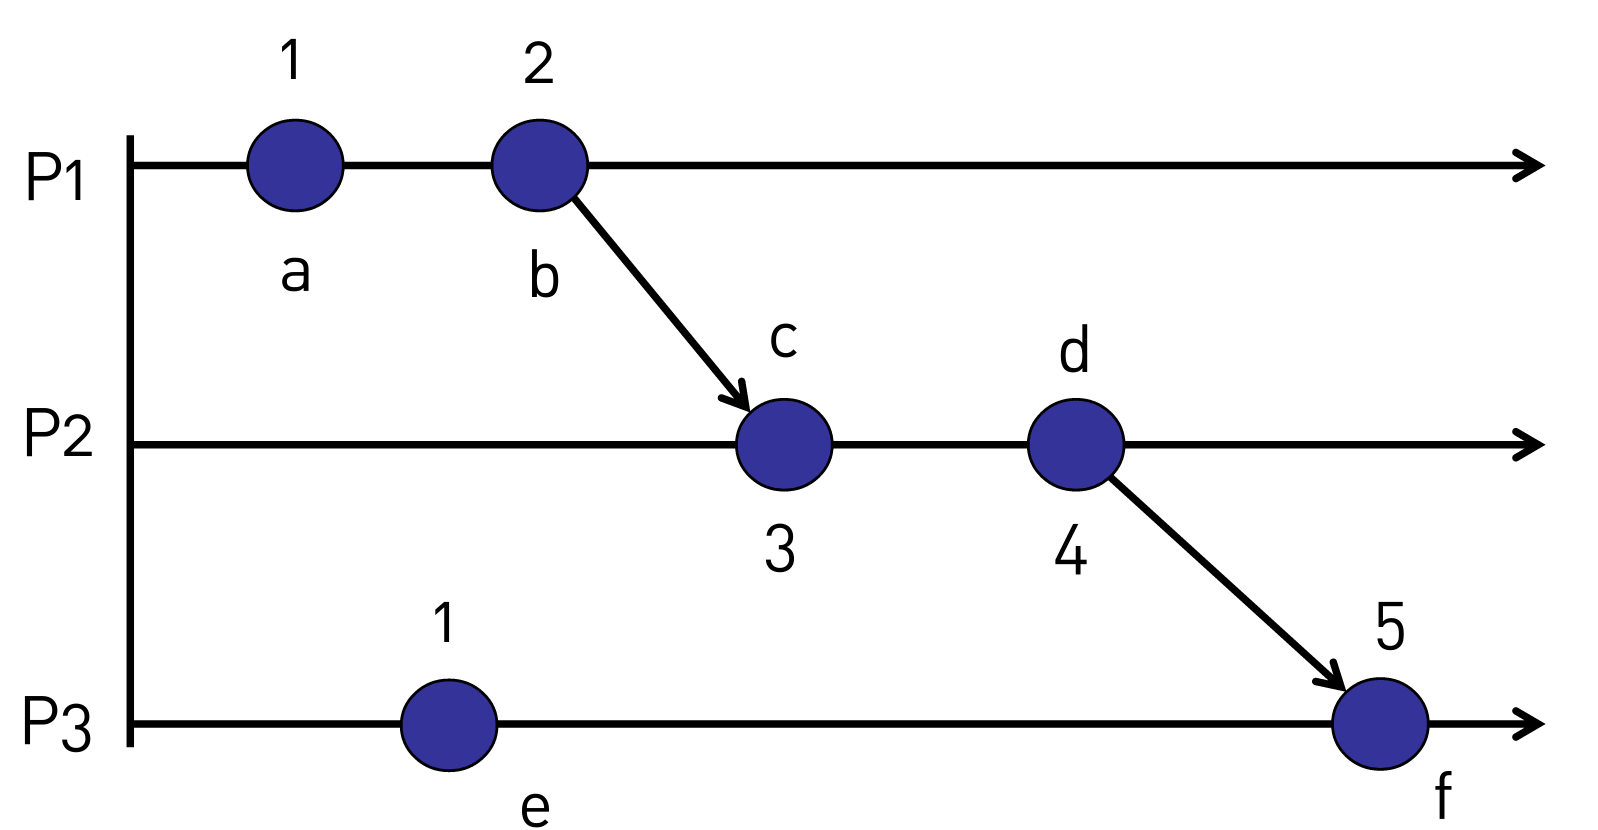
\includegraphics[height=180px]{LamportTime.png}

Die Lamport-Time speichert für jedes Ereignis $e$ einen Integer $L(e)$ , sodass $L(e_{i}) < L(e_{j})$ gilt, falls die Relation "happend before" $e_{i} \rightarrow e_{j}$ gilt. Andersherum gilt aber \textbf{nicht}, dass, wenn $L(e_{i}) < L(e_{j})$ gilt auch $e_{i} \rightarrow e_{j}$ gilt. Die Lamport-Time bildet also die partielle Ordungsrelation  $\rightarrow$ nur korrekt ab, ist aber nicht äquivalent zu ihr. Es gilt also:

\begin{align*}
    e_{i} \rightarrow e_{j} \qquad \Rightarrow \qquad  L(e_{i}) < L(e_{j})         \\
    L(e_{i}) < L(e_{j}) \qquad \cancel{\Rightarrow} \qquad e_{i} \rightarrow e_{j} \\
    e_{i} \rightarrow e_{j} \qquad \cancel{\Leftrightarrow} \qquad L(e_{i}) < L(e_{j})
\end{align*}

Konkret wird die Lamport-Time durch folgende Regeln umgesetzt:
\begin{enumerate}
    \item Zu Beginn stehen alle Zähler für Ereignisse auf 0
    \item Lokale Ereignisse (das schließt Sendeereignisse mit ein) bekommen als Zeit das Inkrement der  Lamport-Time ihres lokalen Vorgängers:\\
          $L(e_{i_{P1}}) = L(e_{i - 1_{P1}}) + 1$
    \item Mit Nachrichten wird die Lamport-Time des zugehörigen Sendeereignisses mitgeschickt
    \item Empfangsereignisse bekommen das Inkrement des Maximums der Lamport-Time ihres lokalen Vorgängers und der Lampert-Time der empfangenen Nachricht:\\
          $L(e_{i_{P1}}) = max(L(e_{i - 1_{P1}}), L(e_{n})) + 1$
\end{enumerate}

\subsubsection{Vector-Time}
\label{sec:vector-time}

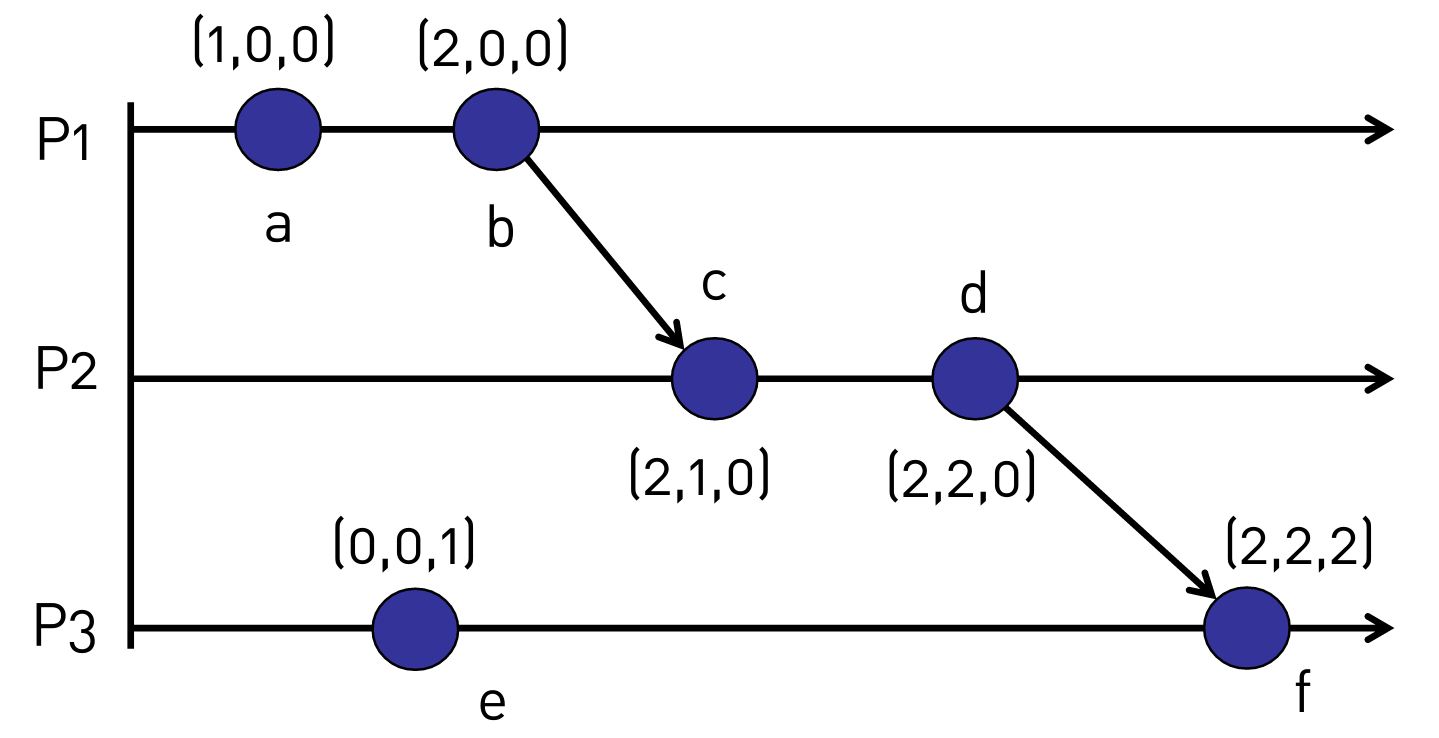
\includegraphics[height=180px]{VectorTime.png}

Die Vector-Time verbessert die \hyperref[sec:lamport-time]{Lamport-Time}, sodass eine kleiner-Relation $<$  über der Menge von Vector-Times äquivalent zur "happened-before"-Relation $\rightarrow$ der Ereignisse ist:
\begin{align*}
    V(e_{i}) < V(e_{j}) \qquad \Leftrightarrow \qquad e_{i} \rightarrow e_{j} \qquad \qquad \qquad \qquad \qquad \qquad \\
    V(e_{i}) = V(e_{j}) \qquad \Leftrightarrow \qquad (V(e_{i}) \quad \cancel{<} \quad V(e_{j})) \quad \wedge \quad (V(e_{j}) \quad \cancel{<} \quad V(e_{i})) \qquad \Leftrightarrow \qquad e_{i} \quad || \quad e_{j}
\end{align*}

Um dies zu erreichen wird für jedes Ereingnis $e$ nicht nur ein Integer gespeichert, sondern ein Vektor von Integern der Dimension $n$, wobei $n$ die Anzahl der Knoten im verteilten System ist und jede Komponente des Vektors einem Knoten zugeordnet wird.\\
Die Kleiner-Relation $<$ ist so, definiert, dass $V(e_{i}) < V(e_{j})$ genau dann gilt, wenn alle Komponenten von $V(e_{i})$ kleiner sind als die entsprechende Komponente in $V(e_{j})$.

Das Zählverfahren ist sehr ähnlich wie bei der Lamport-Time und läuft nach folgenden konkreten Regeln ab:
\begin{enumerate}
    \item Zu Beginn werden alle Komponenten aller Vektoren aller Knoten mit $0$ initialisiert.
    \item Bei lokalen Ereignissen (das schließt Sendeereignisse ein) wird die Komponente des Vektors, die dem eigenen Knoten zugeordnet wird, inkrementiert:\\
          $V_{p_{i}}[p] = V_{p_{i-1}}[p] + 1$
    \item Beim Senden von Nachrichten wird die Vektor-Time des Sendeereignisses mitgeschickt
    \item Beim Empfangen einer Nachricht wird zunächst der eigene Vektor wie in 2. inkrementiert und dann der neue Vektor aus dem Komponentenweise Maximum des eigenen und des empfangenen Vektors gebildet
\end{enumerate}

\subsection{Mutual Exclusion mit Lamport-Time}

In diesem Kapitel soll es darum gehen, wie Mutual Exclusion, also wechselseitiger Ausschluss, in verteilten Systemen realisiert werden kann, so wie es lokal mit Mutexen, die vom OS bereitgestellt werden, funktioniert.\\
Die erste naheliegende Idee ist, es einen zentralen Server zu haben, der die Berechtigung auf eine Ressource zuzugreifen verwaltet. Das ist allerdings mit Blick auf Ausfallsicherheit keine gute Idee. Stattdessen ist es auch möglich die Menge von Requests für den Zugriff auf jedem einzelnen Rechner zu speichern und sicherzustellen, dass für jedes Paar von Requests eindeutig geregelt ist welcher Vorrang hat. Um dies zu bewerkstelligen, wird die \hyperref[sec:lamport-time]{Lamport-Time} \textbf{mit totaler Ordnung} benutzt.\\

Die Vorraussetzungen für die beiden folgenden Algorithmen sind:
\begin{itemize}
    \item Die Nachrichten werden verlustfrei übertragen, d.h. ggf. erneut versendet (z.B. mit TCP)
    \item Die Sendereihenfolge der Nachrichten ist gleich der Empfangsreihenfolge (z.B. mit TCP)
\end{itemize}

\subsubsection{Lamport-Algorithmus}

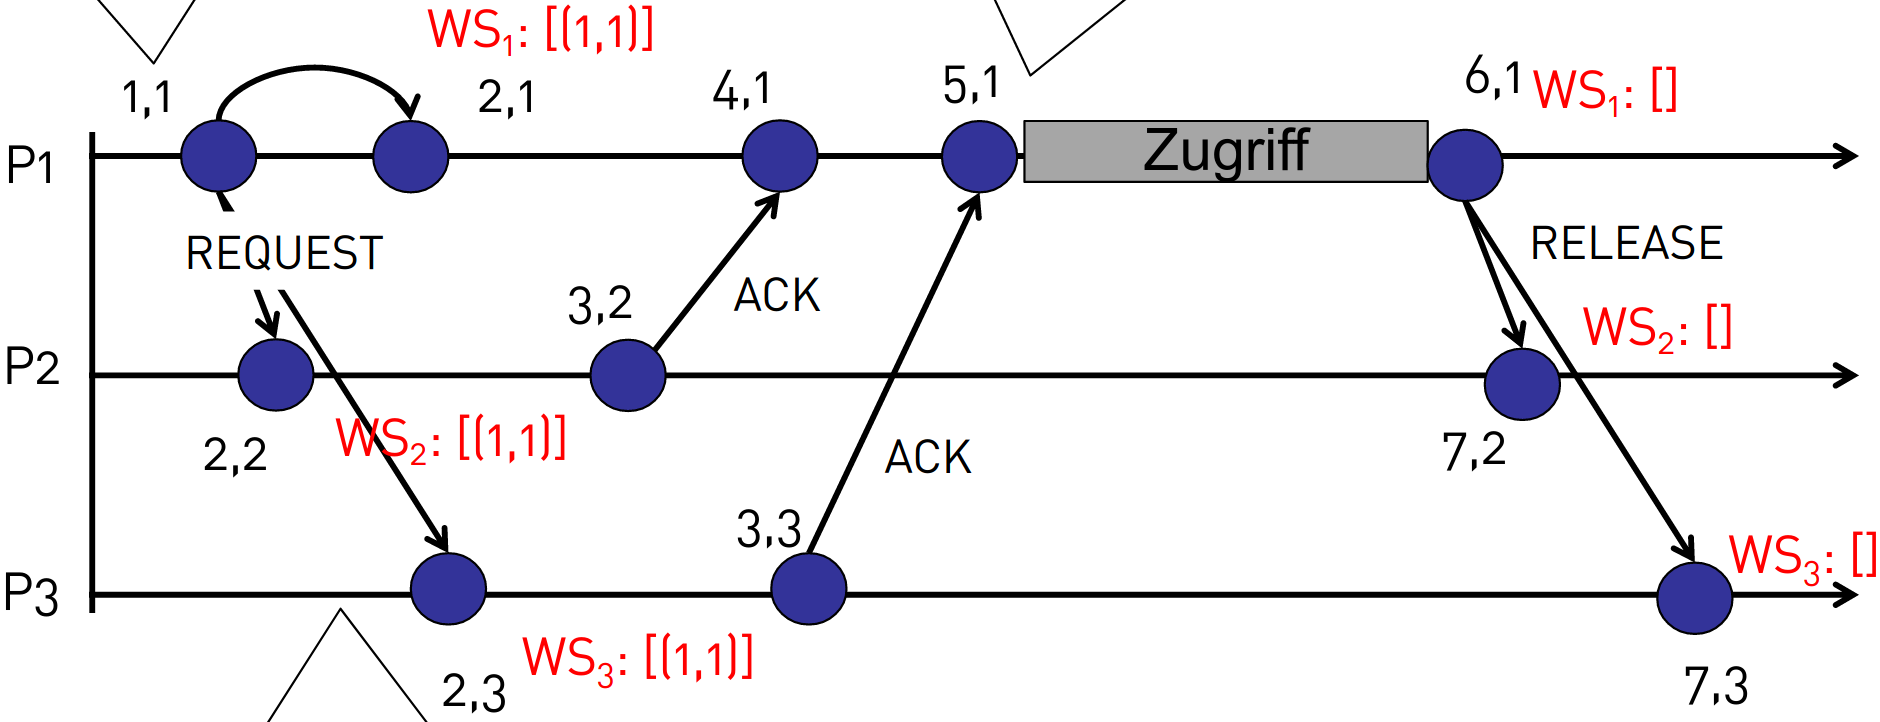
\includegraphics[height=150px]{Lamport-Algorithmus.png}

Beim Lamport-Algorithmus verwaltet jeder Prozess eine lokale Warteschlange mit REQUESTs. Das Vorgehen ist konkret wie folgt definiert:
\begin{enumerate}
    \item Wenn ein Prozess Zugriff auf die Ressource haben möchte, verschickt er ein REQUEST an alle anderen Prozesse
    \item Wenn ein Prozess eine REQUEST erhält, wird diese in die lokale, durch die Lamport-Time total geordnete Liste von REQUESTs eingefügt und \textbf{sofort} ein ACK zurückgesendet
    \item Wenn ein Prozess alle ACK zu seiner REQUEST bekommen hat und seine Request die kleinste Lamport-Time hat, kann er den Zugriff durchführen. Der Prozess kann sich sicher sein, dass es keine Requests mit einer niedrigeren Lamport-Time gibt, die er noch nicht erhalten hat, weil durch die Reihenfolgetreue der Nachrichten keine Nachricht mehr im Netzwerk sein kann, die vor den erhaltenen ACKs verschickt wurde
    \item Wenn ein Prozess seinen Zugriff beendet hat versendet er eine RELEASE Nachricht an alle anderen Prozesse, um die Ressource wieder freizugeben
    \item Wenn ein Prozess eine RELEASE-Nachricht empfängt, entfernt er den zugehörigen Eintrag seiner lokalen Warteschlange
\end{enumerate}

Der Algorithmus verlangt es, dass für jeden Zugriff auf die Ressource $3(n-1)$ Nachrichten versendet werden, wobei $n$ die Zahl der beteiligten Knoten im ist (jeweils ein REQUEST, ACK und RELEASE an alle anderen Knoten).

\subsubsection{Algorithmus von Ricart / Agrawala}

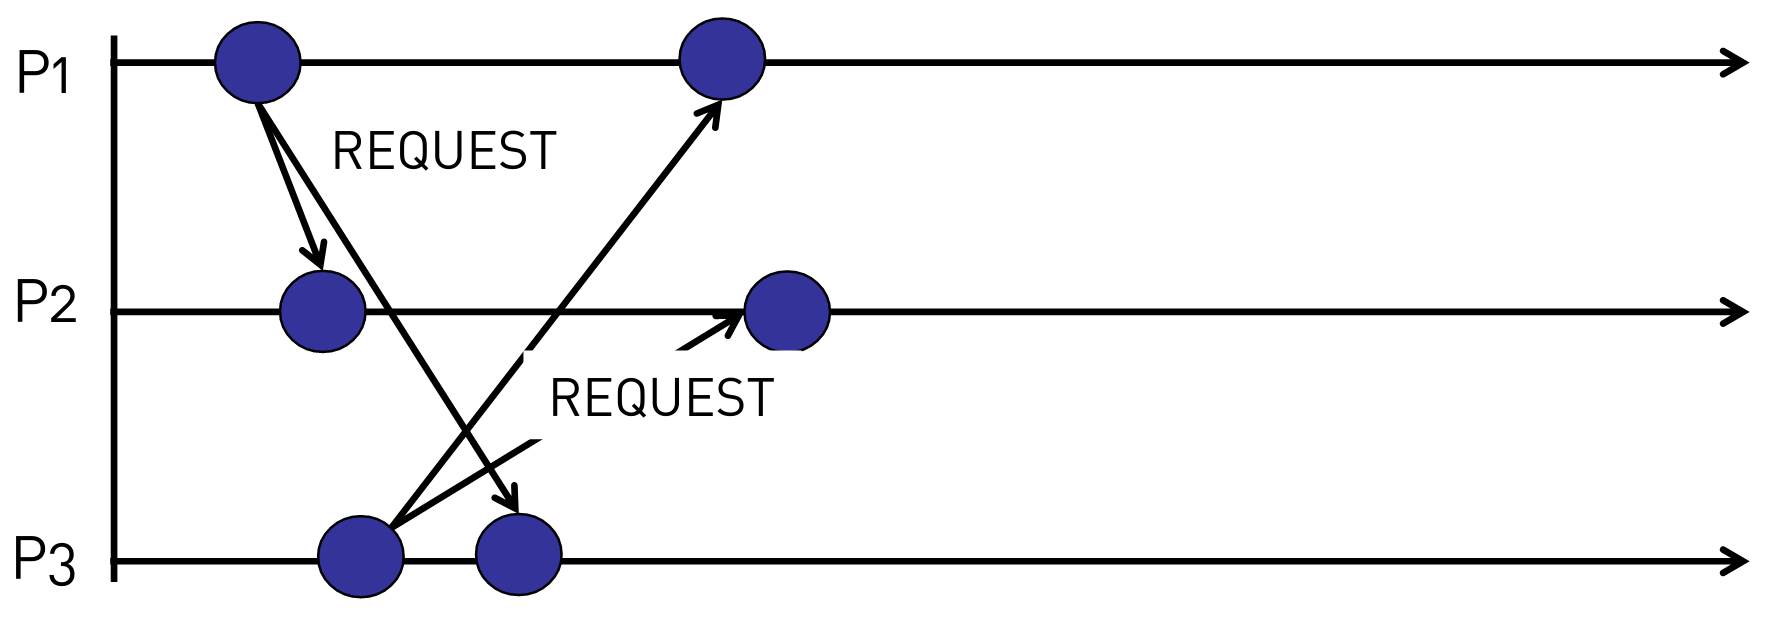
\includegraphics[height=130px]{Ricart-agragawa-algorithmus.png}

Der Algorithmus von Ricart und Argrawala verbessert den Lamport-Algorithmus hinsichtlich seiner Effizienz von $3(n-1)$ Nachrichten auf $2(n-1)$ Nachrichten pro Zugriff. Er modifiziert den Lamport-Algorithmus so, dass nur noch eine REPLY Nachricht anstatt der beiden Nachrichten ACK und RELEASE benötigt wird. Das Vorgehen ist wie folgt definiert:
\begin{enumerate}
    \item Wenn ein Prozess Zugriff auf die Ressource bekommen möchte sendet er ein REQUEST an alle anderen Prozesse (wie bei Lamport-Algorithmus)
    \item Wenn ein Prozess ein REQUEST erhält und selbst noch nicht auf REPLYs wartet (also zurzeit kein Interesse an Zugriff hat) oder die Lamport-Time der eingehenden REQUEST kleiner ist als die der eigenen REQUEST, sendet er sofort ein REPLY
    \item Wenn ein Prozess ein REQUEST erhält und selbst ein REQUEST mit einer kleineren Lamport-Time gesendet hat, sendet er das REPLY erst, wenn er seinen eigenen Zugriff auf die Ressource beendet hat
    \item Wenn ein Prozess alle REPLYs für seine Request erhalten hat, darf er auf die Ressource zugreifen
\end{enumerate}

Auf diese Weise werden erst immer alle REPLYs zu einem REQUEST erhalten, wenn es keine anderen REQUESTs mit einer niedrigeren Lamport-Time gibt. Auf diese Weise hat zu jeder Zeit nur max. 1 Prozess Zugriff auf die Ressource, nämlich der, der die REQUEST mit der niedrigen Lamport-Time gesendet hat.

\subsubsection{Eigenschaften der Algorithmen}

Für den Lamport-Algorithmus und den Algorithmus von Ricart / Agrawala gelten die folgenden Eigenschaften:
\begin{enumerate}
    \item \textbf{Deadlock-Freiheit}\\
          Da durch die totale Ordnung der Requests immer geregelt ist, wer Zugriff hat
    \item \textbf{Starvation-Freiheit}:\\
          Da das Empfangen einer ACK / RESPONSE Nachricht auf einem Knoten $K_{1}$ die eigene Lamport-Time erhöht, ist es für diesen Knoten erst möglich die nächste Response mit einer um $1$ höheren Lamport-Time als die anderen Knoten zu verschicken. Dadurch können auf jeden Fall andere Knoten auch zum Zuge kommen.
\end{enumerate}